\documentclass[11pt]{article}
\topmargin=0.0in %length of margin at the top of the page (1 inch added by default)
\oddsidemargin=0.0in %length of margin on sides for odd pages
\evensidemargin=0in %length of margin on sides for even pages
\textwidth=6.5in %How wide you want your text to be
\marginparwidth=0.5in
\headheight=0pt %1in margins at top and bottom (1 inch is added to this value by default)
\headsep=0pt %Increase to increase white space in between headers and the top of the page
\textheight=9in %How tall the text body is allowed to be on each page

%
\usepackage{makeidx}  % allows for indexgeneration
\usepackage{amsmath}
\usepackage{listings}
\usepackage{algorithm}
\usepackage{algorithmic}
\usepackage{amsthm}
\usepackage{graphicx}

\newtheorem{defn}{Definition}
\newtheorem{lemma}{Lemma}

\lstdefinelanguage{scala}{morekeywords={class,object,trait,extends,with,new,if,while,for,def,val,var,this},
otherkeywords={->,=>},
sensitive=true,
morecomment=[l]{//},
morecomment=[s]{/*}{*/},
morestring=[b]"}
% Default settings for code listings
\lstset{frame=tb,language=scala,aboveskip=3mm,belowskip=3mm,showstringspaces=false,columns=flexible,basicstyle={\small\ttfamily}}
%

\begin{document}

\title{Variant Discovery and Canonicalization via \\ Indexed de Bruijn Graphs}
\author{Frank~Austin~Nothaft, Anthony~D.~Joseph, \and David~A.~Patterson \\
Department of Electrical Engineering and Computer Sciences\\
University of California, Berkeley \\ 
Berkeley, CA 94720, USA \\
\{fnothaft, adj, pattrsn\}@berkeley.edu}

\maketitle              % typeset the title of the contribution

\begin{abstract}

Modern variant calling methods frequently rely on local reassembly based approaches to discover
variants. Although local reassembly allows for the accurate reconstruction of insertion and deletion
variants in the presence of local mapping errors, current reassembly methods provide low throughput.
These methods achieve low throughput due to a reliance on an exhaustive graph search to identify
haplotypes, coupled with the use of expensive realignment methods for haplotype scoring. In this paper,
we enhance the traditional \emph{de Bruijn} graph with the location of $k$-mers in a reference sequence.
First, we demonstrate how an index de Bruijn graph simplifies to an efficient algorithm for local sequence
alignment. We are able to derive canonical edit representations, and achieve $\Omega(n)$ alignment cost
for canonical edits. From this alignment formulation, we demonstrate how an \emph{indexed de Bruijn}
graph can be used for variant discovery in a local reassembly pipeline with lower cost than a traditional
reassembly algorithm. An \emph{indexed de Bruijn} graph has identical storage cost as a traditional
\emph{de Bruijn} graph. 

\end{abstract}

\section{Introduction}
\label{sec:introduction}

The accuracy of insertion and deletion~(INDEL) variant discovery has been improved by the development
of variant callers that couple local reassembly with haplotype-based statistical models to recover INDELs
that were locally misaligned~\cite{albers11}. Now, several prominent variant callers such as the Genome
Analysis Toolkit's~(GATK) \texttt{HaplotypeCaller}~\cite{depristo11}, \texttt{Scalpel}~\cite{narzisi14}, and
\texttt{Platypus}~\cite{rimmer14}. Although haplotype-based methods have enabled more accurate INDEL
and single nucleotide polymorphism~(SNP) calls~\cite{bao14}, this accuracy comes at the cost of
end-to-end runtime~\cite{talwalkar14}. Several recent projects have been focused on improving
reassembly cost either by limiting the percentage of the genome that is reassembled~\cite{bloniarz14} or
by improving the performance of algorithms of the core algorithms used in local
reassembly~\cite{rimmer14}.

The performance issues seen in haplotype reassembly approaches derives from the high asymptotic
complexity of reassembly algorithms. Although specific implementations may vary slightly, a typical
local reassembler performs the following steps:

\begin{enumerate}
\item A \emph{de Bruijn} graph is constructed from the reads aligned to a region of the reference genome,
\item All valid paths~(\emph{haplotypes}) between the start and end of the graph are enumerated,
\item Each read is realigned to each haplotype, typically using a pair Hidden Markov Model~(HMM,
see~\cite{durbin98}),
\item A statistical model uses the read$\leftrightarrow$haplotype alignments to choose the haplotype pair
that most likely represents the variants hypothesized to exist in the region, 
\item The alignments of the reads to the chosen haplotype pair are used to generate statistics that are
then used for genotyping.
\end{enumerate}

In this paper, we focus on steps one through three of the local reassembly problem, as there is wide
variation in the algorithms used in stages four and five~(see~\S\ref{sec:background}). Stage one (graph
creation) has approximately $\mathcal{O}(r l_r)$ time complexity, and stage two (graph elaboration) has
$\mathcal{O}(h \max(l_h))$ time complexity.
The asymptotic time cost bound of this formulation of reassembly comes from stage three, where cost is $\mathcal{O}(h r l_r
\min(l_h))$, where $h$ is the number of haplotypes tested in this region\footnote{The number of
haplotypes tested may be lower than the number of haplotypes reassembled. Several tools
(see~\cite{depristo11,garrison12}) allow users to limit the number of haplotypes evaluated to improve
performance.}, $r$ is the number of reads aligned to this region, $l_r$ is the read length\footnote{For
simplicity, we assume constant read length. This is a reasonable assumption as many of the variant
callers discussed target Illumina reads that have constant length.}, and $\min(l_h)$ is the length of the
shortest haplotype that we are evaluating. This complexity comes from realigning $r$ reads to $h$
haplotypes, where realignment has complexity $\mathcal{O}(l_r l_h)$. We ignore the storage complexity of
reassembly here, but provide an extended
discussion of \emph{de Bruijin} graph complexity in~\S\ref{sec:background}.

In this paper, we introduce the \emph{indexed de Bruijn} graph and demonstrate how it can be used to
reduce the asymptotic complexity of reassembly. An \emph{indexed de Bruijn} graph is identical to a
traditional \emph{de Bruijn} graph, with one modification: when we create the graph, we annotate each
$k$-mer with the index position of that $k$-mer in the sequence it was observed in. This simple addition
enables the use of the \emph{indexed de Bruijn} graph for $\Omega(n)$ local sequence alignment with
canonical edit representations for most edits. This structure can be used for both sequence alignment and
assembly, and achieves a more efficient approach for variant discovery via local reassembly.

\section{Background}
\label{sec:background}

\section{Formulation}
\label{sec:formulation}

To construct an \emph{indexed de Bruijn} graph, we start with the traditional formulation of a \emph{de
Brujin} graph for sequence assembly:

\begin{defn}[de Bruijn Graph]
\label{defn:dbg}
A de Bruijn graph describes the observed transitions between adjacent $k$-mers in a sequence. Each
$k$-mer $s$ represents a $k$-length string, with a $k - 1$ length prefix given by $\text{prefix}(s)$ and a
length 1 suffix given by $\text{suffix}(s)$. We place a directed edge ($\rightarrow$) from $k$-mer $s_1$ to
$k$-mer $s_2$ if $\text{prefix}(s_1)^{\{1, k - 2\}} + \text{suffix}(s_1) = \text{prefix}(s_2)$.
\end{defn}

Now, suppose we have $n$ sequences $\mathcal{S}_1, \dots, \mathcal{S}_n$. Let us assert that for each
$k$-mer $s \in \mathcal{S}_i$, then the output of function $\text{index}_i(s)$ is defined. This function
provides us with the integer position of $s$ in sequence $\mathcal{S}_i$. Further, given two $k$-mers
$s_1, s_2 \in \mathcal{S}_i$, we can define a distance function
$\text{distance}_i(s_1, s_2) = | \text{index}_i(s_1) - \text{index}_i(s_2) |$. To create an \emph{indexed}
de Bruijn graph, we simply annotate each $k$-mer $s$ with the $\text{index}_i(s)$ value for all
$\mathcal{S}_i, i \in \{1, \dots, n\}$ where $s \in \mathcal{S}_i$. This index value is trivial to log when
creating the original \emph{de Bruijn} graph from the provided sequences.

Let us require that all sequences $\mathcal{S}_1, \dots, \mathcal{S}_n$ are not repetitive, which implies
that the resulting de Bruijn graph is acyclic. If we select any two sequences $\mathcal{S}_i$ and
$\mathcal{S}_j$ from $\mathcal{S}_1, \dots, \mathcal{S}_n$ that share at least two $k$-mers $s_1$ and
$s_2$ with common ordering~($s_1 \rightarrow \dots \rightarrow s_2$ in both $\mathcal{S}_i$ and
$\mathcal{S}_j$), the indexed de Bruijn graph $G$ provides several guarantees:

\begin{enumerate}
\item If two sequences $\mathcal{S}_i$ and $\mathcal{S}_j$ share at least two $k$-mers $s_1$ and
$s_2$, we can provably find the maximum edit distance $d$ of the subsequences in $\mathcal{S}_i$ and
$\mathcal{S}_j$, and bound the cost of finding this edit distance at $\mathcal{O}(nd)$,\footnote{Here,
$n = \max(\text{distance}_{\mathcal{S}_i}(s_1, s_2), \text{distance}_{\mathcal{S}_j}(s_1, s_2))$.}
\item For many of the above subsequence pairs, we can bound the cost at $\mathcal{O}(n)$, \emph{and}
provide canonical representations for the necessary edits,
\item $\mathcal{O}(n^2)$ complexity is restricted to aligning the subsequences of $\mathcal{S}_i$ and
$\mathcal{S}_j$ that exist \emph{before} $s_1$ or \emph{after} $s_2$.
\end{enumerate}

Let us focus on cases 1 and 2, where we are looking at the subsequences of $\mathcal{S}_i$ and
$\mathcal{S}_j$ that are between $s_1$ and $s_2$. A trivial case arises when both $\mathcal{S}_i$ and
$\mathcal{S}_j$ contain an identical path between $s_1$ and $s_2$ (i.e.,
$s_1 \rightarrow s_n \rightarrow \dots \rightarrow s_{n + m} \rightarrow s_2$ and
$s_{n + k} \in \mathcal{S}_i \wedge s_{n + k} \in \mathcal{S}_j \forall k \in \{0, \dots , m\}$). Here, the
subsequences are clearly identical. This determination can be made trivially by walking from vertex $s_1$
to vertex $s_2$ with $\mathcal{O}(m)$ cost.

However, three distinct cases can arise whenever $\mathcal{S}_i$ and $\mathcal{S}_j$ diverge between
$s_1$ and $s_2$. For simplicity, let us assume that both paths are independent~(see
Definition~\ref{defn:path-independence}). These three cases correspond to there being either a canonical
substitution edit, a canonical INDEL edit, or a non-canonical (but known distance) edit between
$\mathcal{S}_i$ and $\mathcal{S}_j$.

\begin{defn}[Path Independence]
\label{defn:path-independence}
Given a non-repetitive de Bruijn graph $G$ constructed from $\mathcal{S}_i$ and $\mathcal{S}_j$, we say
that $G$ contains independent paths between $s_1$ and $s_2$ if we can construct two subsets
$\mathcal{S}'_i \subset \mathcal{S}_i, \mathcal{S}'_j \subset \mathcal{S}_j$ of $k$-mers where $s_{i + n}
\in \mathcal{S}'_i \forall n \in \{0, \dots, m_i\}, s_{i + n - 1} \rightarrow s_{i + n} \forall n \in \{1, \dots, m_i\}$,
$s_{j + n} \in \mathcal{S}'_j \forall n \in \{0, \dots, m_j\}, s_{j + n - 1} \rightarrow s_{j + n} \forall n \in \{1,
\dots, m_j\}$, and $s_1 \rightarrow s_i, s_j; s_{i + m_i}, s_{j + m_j} \rightarrow s_2$ and $\mathcal{S}'_i
\bigcap \mathcal{S}'_j = \emptyset$, where $m_i = \text{distance}_{\mathcal{S}_i}(s_1, s_2)$, and $m_j =
\text{distance}_{\mathcal{S}_j}(s_1, s_2)$. This implies that the sequences $\mathcal{S}_i$ and
$\mathcal{S}_j$ are different between $s_1, s_2$,
\end{defn}

We have a canonical substitution edit if $m_i = m_j = k$, where $k$ is the $k$-mer size. Here, we can
prove that the edit between $\mathcal{S}_i$ and $\mathcal{S}_j$ between $s_1, s_2$ is a single base
substitution $k$ letters \emph{after} $\text{index}(s_1)$:

\begin{proof}[Proof regarding Canonical Substitution]
\label{proof:canonical-substitution}
Suppose we have two non-repetitive sequences, $\mathcal{S}_i'$ and $\mathcal{S}_j'$, each of length
$2k + 1$. Let us construct a de Bruijn graph $G$, with $k$-mer length $k$. If each sequence begins with
$k$-mer $s_1$ and ends with $k$-mer $s_2$, then that implies that the first and last $k$ letters of
$\mathcal{S}_i'$ and $\mathcal{S}_j'$ are identical. If both subsequences had the same character at
position $k$, this would imply that both sequences were identical and therefore the two paths between
$s_1, s_2$ would not be independent~(Definition~\ref{defn:path-independence}). If the two letters are
different \emph{and} the subsequences are non-repetitive, each character is responsible for $k$
previously unseen $k$-mers. This is the only possible explanation for the two independent $k$ length
paths between $s_1$ and $s_2$.
\end{proof}

To visualize the graph corresponding to a substitution, take the two example sequences \texttt{CCACTGT}
and \texttt{CCAATGT}. These two sequences differ by a \texttt{C} $\leftrightarrow$ \texttt{A} edit at
position three. With $k$-mer length $k = 3$, this corresponds to the graph in Figure~\ref{fig:sne}.

\begin{figure}[h]
\begin{center}
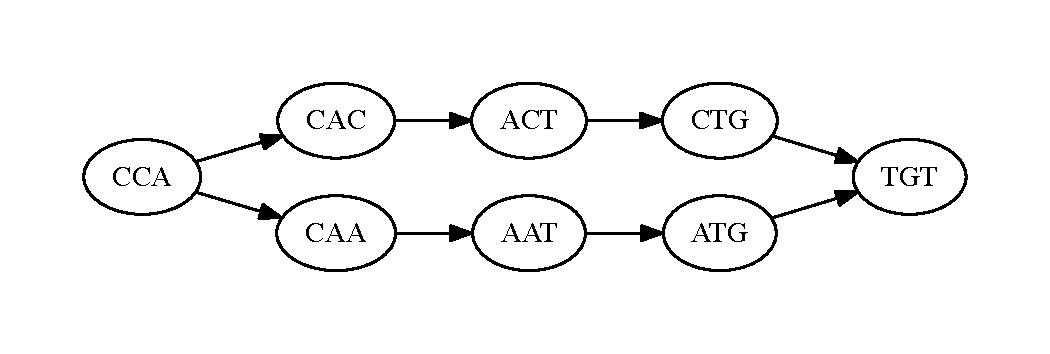
\includegraphics[width=0.5\linewidth, clip=true, trim=0 39 0 39]{graphs/sne.pdf}
\end{center}
\caption{Subgraph Corresponding To a Single Nucleotide Edit}
\label{fig:sne}
\end{figure}

If $m_i = k - 1, m_j \ge k$ or vice versa, we have a canonical INDEL edit (for convenience, we assume
that $\mathcal{S}_i'$ contains the $k - 1$ length path). Here, we can prove that there is a $m_j - m_i$
length insertion\footnote{This is equivalently a $m_j - m_i$ length deletion in $\mathcal{S}_i'$ relative to
$\mathcal{S}_j'$.} in $\mathcal{S}_j'$ relative to $\mathcal{S}_i'$, $k - 1$ letters \emph{after}
$\text{index}(s_1)$:

\begin{lemma}[Distance between $k$ length subsequences]
\label{lem:minimum-distance}
Indexed de Bruijn graphs naturally provide a distance metric for $k$ length substrings. Let us construct an
indexed de Bruijn graph $G$ with $k$-mers of length $k$ from a non-repetitive sequence $\mathcal{S}$.
For any two $k$-mers $s_a, s_b \in \mathcal{S}, s_a \ne s_b$, the
$\text{distance}_\mathcal{S}(s_a, s_b)$ metric is equal to $l_p + 1$, where $l_p$ is the length of the
path (in $k$-mers) between $s_a$ and $s_b$. Thus, $k$-mers with overlap of $k - 1$ have an edge
directly between each other ($l_p = 0$) and a distance metric of 1. Conversely, two $k$-mers that are
adjacent but not overlapping in $\mathcal{S}$ have a distance metric of $k$, which implies $l_p = k - 1$.
\end{lemma}

\begin{proof}[Proof regarding Canonical INDELs]
\label{proof:canonical-indels}
We are given a graph $G$ which is constructed from two non-repetitive sequences $\mathcal{S}_i'$ and
$\mathcal{S}_j'$, where the only two $k$-mers in both $\mathcal{S}_i'$ and $\mathcal{S}_j'$ are $s_1$
and $s_2$ and both sequences provide independent paths between $s_1$ and $s_2$. By
Lemma~\ref{lem:minimum-distance}, if the path from $s_1 \rightarrow \dots \rightarrow s_2 \in
\mathcal{S}_i'$ has length $k - 1$, then $\mathcal{S}_i'$ is a string of length $2k$ that is formed by
concatenating $s_1, s_2$. Now, let us suppose that the path from $s_1 \rightarrow \dots \rightarrow s_2
\in \mathcal{S}_j'$ has length $k + l - 1$. The first $l$ $k$-mers after $s_1$ will introduce a $l$ length
subsequence $\mathcal{L} \subset \mathcal{S}_j', \mathcal{L} \not\subset \mathcal{S}_i'$, and then the
remaining $k - 1$ $k$-mers in the path provide a transition from $\mathcal{L}$ to $s_2$. Therefore,
$\mathcal{S}_j'$ has length of $2k + l$, and is constructed by concatenating $s_1, \mathcal{L}, s_2$.
This provides a canonical placement for the inserted sequence $\mathcal{L}$ in $\mathcal{S}_j'$ between
$s_1$ and $s_2$.
\end{proof}

To visualize the graph corresponding to a canonical INDEL, take the two example sequences
\texttt{CACTGT} and \texttt{CACCATGT}. Here, we have a \texttt{CA} insertion after position two. With
$k$-mer length $k = 3$, this corresponds to the graph in Figure~\ref{fig:indel}.

\begin{figure}[h]
\begin{center}
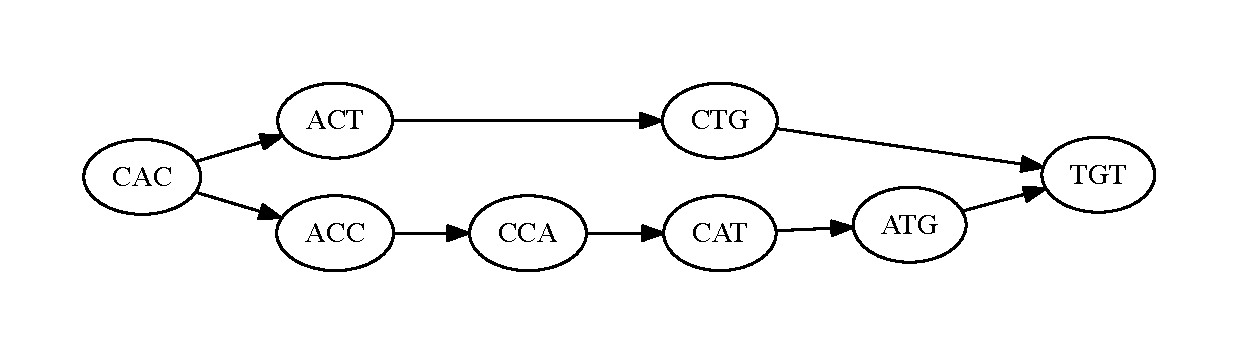
\includegraphics[width=0.5\linewidth, clip=true, trim=0 39 0 39]{graphs/indel.pdf}
\end{center}
\caption{Subgraph Corresponding To a Canonical INDEL Edit}
\label{fig:indel}
\end{figure}

Where we have a canonical allele, the cost of computing the edit is set by the need to walk the graph
linearly from $s_1$ to $s_2$, and is therefore $\mathcal{O}(n)$. However, in practice, we will see
differences that cannot be described as one of the earlier two canonical approaches. First, let us
generalize from the two above proofs: if we have two independent paths between $s_1, s_2$ in the
de Bruijn graph $G$ that was constructed from $\mathcal{S}_i, \mathcal{S}_j$, we can describe
$\mathcal{S}_i$ as a sequence created by concatenating $s_1, \mathcal{L}_i, s_2$.\footnote{This
property holds true for $\mathcal{S}_j$ as well.} The canonical edits merely result from special cases:

\begin{itemize}
\item In a canonical substitution edit, $l_{\mathcal{L}_i} = l_{\mathcal{L}_j} = 1$.
\item In a canonical INDEL edit, $l_{\mathcal{L}_i} = 0, l_{\mathcal{L}_j} \ge 1$.
\end{itemize}

Conceptually, a non-canonical edit occurs when two edits occur within $k$ positions of each other. In
this case, we can trivially fall back on a $O(nm)$ local alignment algorithm~(e.g., a pairwise HMM or
Smith-Waterman, see~\cite{durbin98,smith81}), \emph{but} we only need to locally realign
$\mathcal{L}_i$ against $\mathcal{L}_j$, which reduces the size of the realignment problem. However, we
can further limit this bound by limiting the maximum number of INDEL edits to $d = | l_{\mathcal{L}_i} -
l_{\mathcal{L}_j} |$. This allows us to use an alignment algorithm that limits the number of INDEL
edits~(e.g., Ukkonen's algorithm~\cite{ukkonen85}). By this, we can achieve $O(n(d + 1))$ cost.

\section{Specialization for Local Reassembly}
\label{sec:local-reassembly}

As stated in~\S\ref{sec:formulation}, we have assumed that we want to find the edits between two or
more \emph{known} sequences. However, when performing local reassembly for variant discovery/calling,
our goal is to identify all possible variants and to associate probabilities to observations that contain these
variants. This hypothesized variants are generated by examining the reads aligned to the reference
at/near a given site.

However, we can adopt a ``pooled'' model that uses the indexed de Bruijn graph to discover alternate
alleles without performing a search for all haplotypes. Here, we extract a substring $\mathcal{R}$ from a
reference assembly, corresponding to the subsection of that reference that we would like to reassemble.
Then, we create a pooled ``sequence'' $\mathcal{P}$, that is generated from the $k$-mers present in
the reads aligned to $\mathcal{R}$. However, since $\mathcal{P}$ is a composite of the pooled reads, we
cannot assign indices to $k$-mers in $\mathcal{P}$. Instead, we will rely wholly on the path length
properties demonstrated in~\S\ref{sec:formulation} and the indices of $k$-mers in $\mathcal{R}$ to
discover and anchor alleles. First, let us classify paths where $\mathcal{R}$ and $\mathcal{P}$ diverge
into two types:

\begin{itemize}
\item \textbf{Spurs:} A spur is a set $S$ of $n$ $k$-mers $\{s_1, \dots, s_n\}$ where either $s_1$ or
$s_n \in \mathcal{R}, \mathcal{P}$ and all other $k$-mers are $\not\in \mathcal{R}, \in \mathcal{P}$,
and where $s_i \rightarrow s_{i + 1} \forall i \in \{1, \dots, n - 1\}$. If $s_1 \in \mathcal{R}$, then $s_n$ must 
not have a successor. Alternatively, if $s_n \in \mathcal{R}$, than $s_1$ is required to not have a
predecessor.
\item \textbf{Bubbles:} A bubble is a set $S$ of $n$ $k$-mers $\{s_1, \dots, s_n\}$ where both $s_1$ and
$s_n \in \mathcal{R}, \mathcal{P}$ and all other $k$-mers are $\not\in \mathcal{R}, \in \mathcal{P}$, and
where $s_i \rightarrow s_{i + 1} \forall i \in \{1, \dots, n - 1\}$.
\end{itemize}

Currently, we disregard spurs. Spurs typically result from sequencing errors near the start or end of a
read. Additionally, given a spur, we cannot put a constraint on what sort of edit it may be from the
reference, which increases the computational complexity of processing the spur. We concede that this
may not be the best approach, and have included a longer discussion of the accuracy impact of this
decision, as well as options for processing spurs with an indexed de Bruijn graph in~\S\ref{sec:spurs}.

We can elaborate the graph and identify variants by walking the graph from the first $k$-mer in
$\mathcal{R}$. Although haplotype elaboration algorithms have $\mathcal{O}(nh)$ cost where
$n = V(G)$ and $h$ is the number of haplotypes described by the graph, we can limit our graph traversal
to have $\mathcal{O}(n)$ cost by introducing a tail-recursive finite state machine~(FSM). Whenever we
reach a branch point in the graph, our FSM will push state onto a stack, which allows us---with a few
exceptions---to avoid making multiple traversals through a single $k$-mer in the graph. Our FSM has
the following states:

\begin{itemize}
\item \texttt{R}, \texttt{Reference}: We are on a run of $k$-mers that are in $\mathcal{R}$.
\item \texttt{A}, \texttt{Allele}: We are on a run of $k$-mers that have diverged off of the reference. We
have a divergence start point, but have not connected back to the reference yet. This could be either
a bubble or a spur. 
\item \texttt{C}, \texttt{ClosedAllele}: We were on a run of $k$-mers that had diverged off of the reference,
but have just reconnected back to the reference and now know the start and end positions~(in
$\mathcal{R}$) of the bubble, as well as the non-reference sequence and length of the bubble.
\end{itemize}

We allow the FSM to make the following state transitions, which are depicted in Figure~\ref{fig:fsm}:

\begin{itemize}
\item \texttt{R} $\rightarrow$ \texttt{R}: We are continuing along a reference run.
\item \texttt{R} $\rightarrow$ \texttt{A}: We were at a $k$-mer $\in \mathcal{R}$, and have seen a branch
to a $k$-mer $\not\in \mathcal{R}$.
\item \texttt{A} $\rightarrow$ \texttt{A}: We are continuing along a non-reference run.
\item \texttt{A} $\rightarrow$ \texttt{C}: We were on a non-reference run, and have just connected back to
a reference $k$-mer.
\item \texttt{C} $\rightarrow$ \texttt{R}: We have just closed out an allele, and are back at a $k$-mer
$\in \mathcal{R}$.
\end{itemize}

\begin{figure}[h]
\begin{center}
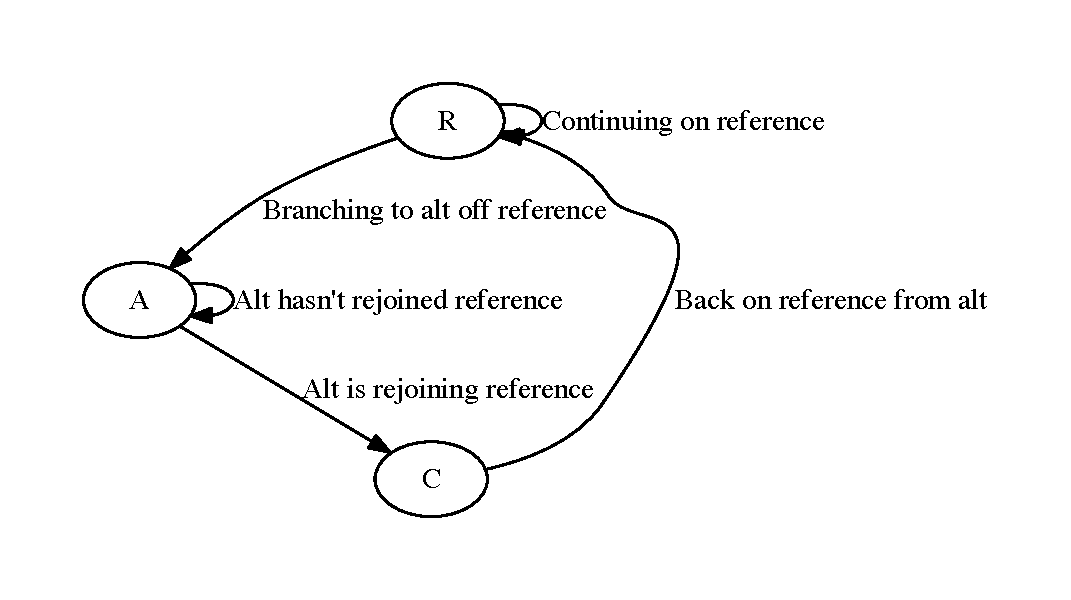
\includegraphics[width=0.5\linewidth, clip=true, trim=0 39 0 39]{graphs/fsm.pdf}
\end{center}
\caption{Finite State Machine for Pooled vs. Reference Assembly}
\label{fig:fsm}
\end{figure}

We initialize the state machine to \texttt{R}, and start processing with the first $k$-mer from $\mathcal{R}$.
Per $k$-mer, we evaluate the possible state transitions of each successor $k$-mer. If the set of successor
$k$-mers contains a single $k$-mer, we continue to that state. If the successor set contains multiple
$k$-mers, we choose a successor state to transition to, and push the branch context of all other
successor states onto our stack. If the successor set is empty, we pop a branch context off of the stack,
and switch to that context. We stop once we reach a $k$-mer whose successor set is empty, \emph{and}
our branch context stack is empty.

The implementation of the \texttt{R} and \texttt{A} states largely amount to bookkeeping. In the \texttt{R}
state, we must track the current position in $\mathcal{R}$, and in \texttt{A}, we must record where we
branched off of $\mathcal{R}$, and $\mathcal{L}'$, the bases we have seen since we
branched\footnote{Although we are processing $k$-mers, we only need to reconstruct the sequence that
the $k$-mers are describing by taking the first base from each successive $k$-mer.} off of $\mathcal{R}$.
If we are in the \texttt{A} state and walk to a $k$-mer $\in \mathcal{R}$, we then transition into the
\texttt{C} state. Using the positions of our branch point and the current $k$-mer in $\mathcal{R}$, we are
able to calculate the length of the reference path via Lemma~\ref{lem:minimum-distance}, while the length
of the non-reference path is given by $l_{\mathcal{L}'}$. The edited sequence $\mathcal{L}$ present
between the branch point and the current $k$-mer is given by trimming the first $k - 1$ bases from
$\mathcal{L}'$. If we have a non-canonical edit, or a deletion in $\mathcal{P}$ relative to $\mathcal{R}$,
we can look these bases up by indexing into $\mathcal{R}$.

To improve computational efficiency, we should emit statistics for genotyping \emph{while} traversing the graph. By doing
this, we can eliminate the need for realignment in haplotype reassembly. Since we have constructed a
graph where every $k$-mer is anchored to a reference position or to a position in a variant, or is in a spur,
if we log several statistics when processing reads from $\mathcal{P}$, we can directly emit the probability
observations that support a reference base or a variant allele. Although the relevant statistics vary
between different variant calling/genotyping algorithms, common statistics include base and mapping
quality, as well as strand of the observation. Additionally, genotyping algorithms that incorporate phasing
may want to identify observations that came from the same allele. These statistics can be logged when
chopping the reads in $\mathcal{P}$ into $k$-mers at a low cost.

As noted earlier in this section, we normally do \emph{not} need to retrace through any $k$-mers in the
graph when processing the graph. However, we may need to retrace $k$-mers if we have overlapping
variants. For example, take the reference string \texttt{ACTGCCGTCT}, the SNV \texttt{ACTGCAGTCT},
and the complex variant \texttt{ACTGCAAGTCT}\footnote{At \texttt{CCG}, we have inserted an \texttt{A}
between the two \texttt{C}s, and changed the second \texttt{C} $\rightarrow$ \texttt{A}. Alternatively, this
can be described as a deletion of the second \texttt{C} and an insertion of \texttt{AA} between
\texttt{CG}.}. For $k = 4$, both variants share the 4-mer \texttt{AGTC}, but both take independent paths
from the reference 4-mer \texttt{CTGC} to \texttt{AGTC}. In this case, we need to walk \texttt{AGTC} twice.

\section{Discussion and Future Work}
\label{sec:discussion}

In this work, we have presented algorithms that allow for efficient sequence comparison using an indexed
de Bruijn graph, and have then demonstrated how this can be used in a local reassembly pipeline. We are
working to build a variant calling and genotyping platform using this algorithm, and hope to demonstrate
results on real data soon.

One limitation of current local reassemblers is that they cannot simultaneously reassemble two regions
of the reference genome. This strategy \emph{may} be useful if we have two regions $\mathcal{R}_1$ and
$\mathcal{R}_2$ with high similarity. Since a global aligner may not properly place reads into
$\mathcal{R}_1$ or $\mathcal{R}_2$ during alignment, the reads aligned to $\mathcal{R}_1$ and
$\mathcal{R}_2$ could be placed into the same pool $\mathcal{P}$ for reassembly. By emitting putative
variants from this graph \emph{and} using a genotyping model that incorporated phasing, this structure
may be able to correct for global alignment errors between similar regions. Pooling multiple regions
together can be used for detecting structural variants. If graph $G$ constructed from $\mathcal{R}_1,
\mathcal{R}_2, \mathcal{P}$ contains an arc $s_0 \rightarrow \dots \rightarrow s_n$ where $s_i \in
\mathcal{P}, \not\in \mathcal{R}_1, \mathcal{R}_2, \forall i \in \{1, \dots, n - 1\}$ and $s_0 \in \mathcal{P},
\mathcal{R}_1, \not\in \mathcal{R}_2, s_n \in \mathcal{P}, \mathcal{R}_2, \not\in \mathcal{R}_1$, then the
arc from $s_1$ to $s_n$ identifies a possible structural variant breakpoint between $\mathcal{R}_1$ and
$\mathcal{R}_2$.

Although this paper motivates the use of indexed de Bruijn graphs for variant calling, they can also
be used for canonicalizing the output of multiple variant calling tools. Specifically, assume that we have
two variants that are within $n$ bases of each other. For these two variants, we can generate sequences
$\mathcal{V}_1, \mathcal{V}_2$ by substituting the variant into $\mathcal{R}$ overlapping the site. We
can then construct an indexed de Bruijn graph from $\mathcal{V}_1, \mathcal{V}_2$ with $k$-mer length
$k \ge n$. If both $\mathcal{V}_1, \mathcal{V}_2$ overhang the variants by $\ge k$ bases and the graph
contains a single path, the two variant representations are equivalent. This presents a more principled
strategy for canonicalizing variants than the \textsc{Rescue} strategy used in the \texttt{SMASH}
benchmarking suite~\cite{talwalkar14}.

\subsection{Limits of Processing Repeated Sequences}
\label{sec:limits-repeated-sequences}

In this paper, we constrain our sequences to not contain repeated subsequences of length greater than
$k$, where $k$ is the $k$-mer length used when constructing a de Bruijn graph $G$. If there is a repeated 
subsequence with length $\ge k$, then $G$ will contain a cycle. Although \emph{de novo} assembly
methods attempt to resolve repeats through scaffolding~\cite{zerbino09}, local reassembly methods
frequently disallow repeats. Both the GATK's \texttt{HaplotypeCaller}~\cite{depristo11} and
\texttt{Scalpel}~\cite{narzisi14} increment the $k$-mer size until the repeat is eliminated or the tool
gives up on locally reassembling the region.

\subsection{Methods for Processing Spurs}
\label{sec:spurs}

Although local reassembly methods typically trim spurs from the haplotype reassembly graph to reduce
the graph's complexity, the statistics from the bases in these spurs are assigned to locations on a
haplotype during the realignment phase and are captured during genotyping/variant calling. Thus, in
practice, we would like to place spurs in our graph as an small edit off of the reference genome or of an
arc in $\mathcal{P}$. Note that a spur is created whenever a sequencing error occurs within $k$ bases of
the start or end of a read. Although we suggest exact realignment in~\S\ref{sec:formulation}, we expect
errors in Illumina data to be single nucleotide errors, and thus searching for a single nucleotide
substitution edit should suffice. If the spur branches off of a path in $\mathcal{R}$, then it is likely best to
realign the spur to $\mathcal{R}$. If the spur branches off of a divergent variant within $k$ bases of the
variant either branching off of or rejoining $\mathcal{R}$, then we can realign the spur to the remainder of
the variant's path, plus any necessary bases from $\mathcal{R}$.

\section{Conclusion}
\label{sec:conclusion}

In this paper, we have introduced the \emph{indexed de Bruijn} graph. This extension of the traditional
\emph{de Bruijn} graph allows for $\Omega(n)$ local alignment of two or more sequences, with a hard
$\mathcal{O}(n)$ bound for canonical edits and an $\mathcal{O}(l^2)$ bound for non-canonical edits
(in genotyping, $l$ is the variant allele length, which is typically much smaller than $n$). After describing this structure, we have demonstrated how
indexed de Bruijn graphs can be used with a pooled model to locally reassemble haplotypes that contain
variants. By using an indexed de Bruijn graph, we are able to reduce the runtime complexity of the local
reassembly algorithms that are commonly used for variant discovery and calling.

\bibliographystyle{acm}
\bibliography{reference-threaded-debruijn}

\end{document}
